\section{\sysname{} Design}
\label{sec:system}

\sysname{} avoids the problems with manual policies or application-specific
solutions by structuring adaptation as a set of approximate, modular and
extensible specifications, or APIs (\autoref{sec:struct-adapt}). The
well-defined structure allowed us to build a generic profiling tool that learns
an accurate relationship (the profile) between bandwidth consumption and
application accuracy (\autoref{sec:automatic-profiling}). The accurate profile
then allows the runtime to react with precision: achieving low latency and high
accuracy when facing bandwidth variation
(\autoref{sec:runtime}). \autoref{fig:overview} shows the high-level overview of
\sysname{}.

\begin{figure}
  \centering
  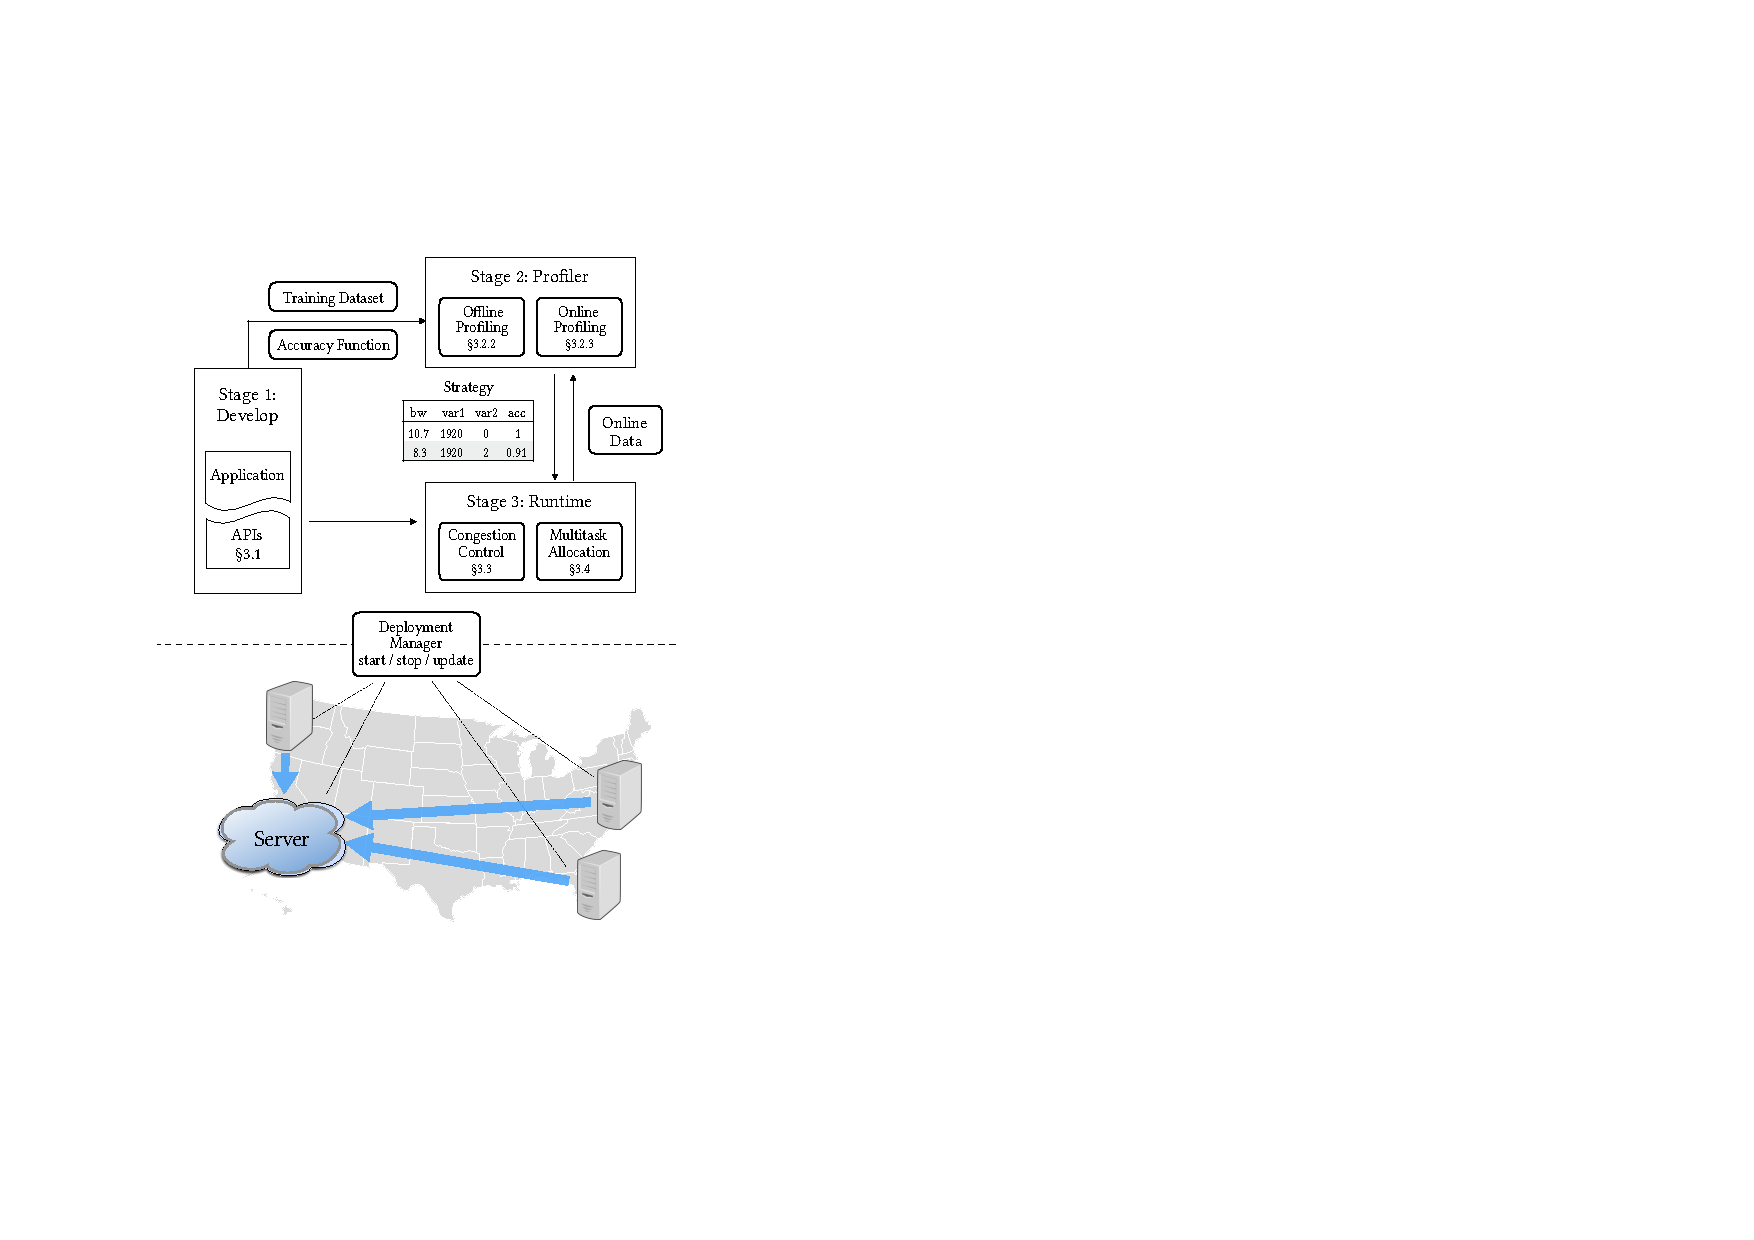
\includegraphics[width=0.9\linewidth]{figures/system.pdf}
  \caption{High-level overview of \sysname{}.}
  \label{fig:overview}
\end{figure}

\begin{table*}
  \small
  \centering
  \begin{tabular}{ c r l }
    \toprule
    \multirow{5}{*}{Normal Operators}
    & \textit{map} (f: I $\Rightarrow$ O) & Stream<I> $\Rightarrow$ Stream<O> \\
    & \textit{skip} (i: Integer) & Stream<I> $\Rightarrow$
                                   Stream<I> \\
    & \textit{sliding\_window} (count: Integer, f: Vec<I> $\Rightarrow$ O) & Stream<I> $\Rightarrow$
                                                                            Stream<O> \\
    % & \textit{tumbling\_window} (count: Integer, f: Vec<I> $\Rightarrow$ O) & Stream<I> $\Rightarrow$
    %                                                                          Stream<O> \\
    & \textit{timed\_window} (time: Duration, f: Vec<I> $\Rightarrow$ O) & Stream<I> $\Rightarrow$
                                                                          Stream<O> \\
    & ... & ... \\
    \midrule
    \multirow{5}{*}{Degradation Operators}
    & \textit{maybe} (knobs: Vec<T>, f:  (T, I) $\Rightarrow$ I) & Stream<I> $\Rightarrow$
                                                                 Stream<I> \\
    & \textit{maybe\_skip} (knobs: Vec<Integer>) & Stream<I> $\Rightarrow$ Stream<I> \\
    & \textit{maybe\_head} (knobs: Vec<Integer>) & Stream<Vec<I>{}> $\Rightarrow$
                                                   Stream<Vec<I>{}> \\
    & \textit{maybe\_downsample} (knobs: Vec<(Integer, Interger)>) & Stream<Image> $\Rightarrow$ Stream<Image> \\
    & ... & ... \\
    \bottomrule
  \end{tabular}
  \caption{Stream processing operators in \sysname{}. \texttt{Vec<T>} represents
    a list of elements with type \texttt{T}.}
  \label{tab:operators}
\end{table*}

\subsection{APIs for Structured Adaptation}
\label{sec:struct-adapt}

%% Introduce graphs of operators model
The majority of stream processing applications today are constructed as a
directed graph of operators~\cite{toshniwal2014storm, zaharia2013discretized},
where each operator transforms input streams into new streams. \sysname{}
borrows the same computation model. We list some example operators, such as
\texttt{map} and \texttt{skip}, in \autoref{tab:operators}.

Along with normal operators, \sysname{} integrates special \maybe{} operators
that degrades the data quality, yielding potential bandwidth savings. Our design
has the following goals: (i) to free developers from specifying exact rules, the
API should tolerate approximate specifications; (ii) to allow combining multiple
dimensions, the API should be modular: each operator is a unit and developer can
chain multiple operators; (iii) to support flexible integration with arbitrary
degradation functions, the API should take user-defined functions
(UDFs). Therefore, our API is,
\vspace{-2pt}
\begin{lstlisting}
        maybe(knobs: Vec<T>, f: (T, I) => I)
\end{lstlisting}

We illustrate the usage of \texttt{maybe} operator with an example that
quantizes a stream of integers in Rust:

\vspace{-2pt}
\begin{lstlisting}
    let quantized_stream = vec![1, 2, 3, 4].into_stream()
        .maybe(vec![2, 4], |k, p| p.wrapping_div(k));
        .collect();
\end{lstlisting}

The snippet creates a stream of integers, chains a degradation operation and
collects the execution result. In this example, the knob is [2, 4], and the
degradation function performs a wrapping (modular) division where the divisor is
the chosen knob. The knob value modifies the quantization level, affecting the
output: [1, 2, 3, 4] (no degradation), [0, 1, 1, 2] (k=2), or [0, 0, 0, 1]
(k=4). If the stream is subsequently encoded---for example, run-length encoding
as in JPEG~\cite{wallace1992jpeg}---for transmission, the bandwidth consumption
will change according to the level of degradation.

Based on the \texttt{maybe} primitive, one can implement wrappers of degradation
operations for common data types. For instance, \texttt{maybe\_head} will
optionally takes the top values of the \textit{list}; and
\texttt{maybe\_downsample} can adjust the \textit{image} resolution to a
configured target. \sysname{} provides a few such operations as libraries for
developers (\autoref{tab:operators}).

With our APIs, the example mentioned in \autoref{sec:making-case-sys-approach}
can now be implemented as follows:

\vspace{-2pt}
\begin{lstlisting}[caption={Video Processing Example}, label={lst:ex}]
   let app = Camera::new((1920, 1080, 30))
      .maybe_downsample(vec![(1600, 900), (1280, 720)])
      .maybe_skip(vec![2, 5])
      .map(|frame| frame.show())
      .compose();
\end{lstlisting}

This snippet first instantiates a \texttt{Camera} source, which produces
\texttt{Stream<Image>} with 1920x1080 resolution and 30 FPS. Two degradation
operations follow the source: one that downsamples image to either 1600x900 or
1280x720 resolution; one that skips frames with a parameter of 2 or 5, resulting
in 30/(2+1)=10 FPS or 30/(5+1)= 6 FPS. In this example, degraded images are
shown on the display, while in practice, further processing, such as encoding
and transmission, operators can be chained.

Structured adaptation not only simplifies the specifications of degradation, the
structure also facilitates learning an accurate profile
(\autoref{sec:automatic-profiling}) and reacting at runtime
(\autoref{sec:runtime}).

%%% Local Variables:
%%% mode: latex
%%% TeX-master: "sosp17"
%%% End:

\subsection{Automatic Profiling}
\label{sec:automatic-profiling}

The goal of the profiling is to learn how different levels of degradation
affects the bandwidth demand and application accuracy. By exploring this
trade-off space, \sysname{} generates a Pareto-optimal \textit{profile} for each
application. We formulate the profiling and discuss the designs for offline and
online profiling.

\subsubsection{Profiling Formalism}
\label{sec:formalize-profiling}

Suppose in a stream processing application that $n$ \maybe{} operators are
used. Each introduces a knob $k_i$. We assume these operators are independent
from each other; their combination forms a \textit{configuration}
$c = [k_{1}, k_{2}, ... k_{n}]$. The set of all possible configurations
$\mathbb{C}$ is the space that our profiling system needs to explore. For each
configuration $c$, there are two mappings that our system needs to explore: a
mapping from $c$ to its bandwidth requirement $B(c)$ and its accuracy measure
$A(c)$. \autoref{tab:notations} summarizes the symbols used in this paper.

The Pareto-optimal set $\mathbb{P}$ is then defined (\autoref{eq:pareto}): for
all $c \in \mathbb{P}$, there is no alternative configuration $c'$ that requires
less bandwidth while giving a higher accuracy.

{\small
\begin{equation}
  \mathbb{P} = \{ c \in \mathbb{C} : \{ c' \in \mathbb{C}: B(c') < B(c),
  A(c') > A(c) \} = \varnothing\}
  \label{eq:pareto}
\end{equation}
}%

\begin{table}
  \small
  \centering
  \begin{tabular}{r l}
    \toprule
    \textbf{Symbol} & \textbf{Description} \\
    \midrule
    $n$ & number of degradation operations \\
    $k_i$ & the \textit{i}-th degradation knob \\
    $c = [k_{1}, k_{2}, ... k_{n}]$ & one specific configuration \\
    $\mathbb{C}$ & the set of all configurations \\
    \midrule
    $B(c)$ & bandwidth requirement for $c$ \\
    $A(c)$ & accuracy measure for $c$ \\
    $\mathbb{P}$ & Pareto efficienct set \\
    \bottomrule
  \end{tabular}
  \caption{Notations used in profiling (keep?).}
  \label{tab:notations}
\end{table}

Since there is often no closed form relation for $B(c)$ and $A(c)$, our system
takes a data-driven approach: with a representative training dataset and an
application-specific utility function, our system evaluates each configuration
for its bandwidth and accuracy. The accuracy can either be measured against the
groundtruth; or in the case when labelled dataset is not available, \sysname{}
uses the results when all degradations are turned off as the reference. We will
discuss concrete knobs, configurations, $B(c)$ and $A(c)$ when we present the
example applications in \autoref{sec:build-appl}.

\subsubsection{Offline Profiling}
\label{sec:offline-profiling}

The offline profiling requires an exhaustive search. Developers using \sysname{}
will first perform an offline profiling that generates the Pareto-optimal
profile by supplying training dataset and application accuracy function. Because
our APIs are general, there is no restriction in the values or functions
provided for \maybe{}. Without \textit{a prior}, any configuration is possible
to be inside the optimal profile.

The exhaustive search is expensive. Therefore, the offline profiling requires to
explore the entire parameter space, which is a combinatorial space of all
knobs. For \textit{offline}, the time required is acceptable.

We note that parallelism is usable for profiling. Except for the groundtruth (or
reference label), two different configurations have no dependence over each
other. Making the profiling an embarrassingly parallel task.

cite ernest experiment design.

\subsubsection{Online Profiling}
\label{sec:online-profiling}

The offline profile is susceptible to ``model drift''. When the required
bandwidth is underestimated, data will be queued at the sender and application
latency will increase. When the accuracy is incorrectly measured, the actual
application performance will be suboptimal. The drift needs to be corrected
online. There are two particular challenges for online profiling.

The first is the lack of groundtruth data or reference data. During the online
execution, it's often infeasible to get labelled data as the groundtruth. For
example, image labelling is known to be labor intensive and time
consuming~\cite{russell2008labelme}. In addition, the original un-degraded data
need to be transmitted from the sender. \sysname{} addresses labelling by using
the un-degraded data as the reference and allocate additional bandwidth for
backhaulling portions of the un-degraded data. While the additional bandwidth
seems a waste, in our design, during the runtime's probing phase, the original
data can enjoy a free ride. Details of the probing is in \autoref{sec:runtime}.

The second challenge is how to profile efficiently. We use the offline profiling
information as a prior to speed-up the online profiler. Specficially, we employ
two techniques: degradation-aware parallelization and partial profiling.

\para{Degradation-aware parallelization:} The profiling tasks of exploring all
configurations are easily parallelizable. Normal job schedulers don't assume the
knowledge of estimated task completion time, therefore the parallel execution
suffers from sub-optimal assignments. Aided with the offline profiling
statistics (the time it requires to profile a particular configuration), we can
schedule the online profiling tasks with a longest first scheduling that
minimizes the makespan.

\para{Partial profiling:} In time domain, the profiling could use a smaller
chunk of data to approximate the best strategy. Besides, we can profiling a
subset of the total configurations and measures its difference from the current
profile. If the difference exceeds a certain threshold, it triggers a full
profiling.

%%% Local Variables:
%%% mode: latex
%%% TeX-master: "sosp17"
%%% End:

\subsection{Runtime Adaptation}
\label{sec:runtime}

\begin{figure}
  \centering
  \resizebox{\columnwidth}{!}{
    \begin{tikzpicture}
  %
  % Define basic styles
  %
  % Node
  \tikzstyle{module} = [draw, very thick, rounded corners,
  fill=white, minimum height=2.5em, inner sep=0.5em,
  rectangle, font={\bfseries}, align=center]
  \tikzstyle{cmodule} = [module, fill=black!20]

  % Edge
  \tikzstyle{stateEdgePortion} = [black, thick];
  \tikzstyle{dataEdge} = [stateEdgePortion, ->];
  \tikzstyle{controlEdgePartial} = [stateEdgePortion, dashed];
  \tikzstyle{controlEdge} = [controlEdgePartial, ->];
  \tikzstyle{controlDoubleEdge} = [controlEdgePartial, <->];
  \tikzstyle{edgeLabel} = [pos=0.5, text centered, font={\itshape}];

  \node[name=client, draw, very thick, fill=white,
  double copy shadow={shadow xshift=2pt, shadow yshift=-2pt, fill=white, draw},
  text height=13em, text width=31.5em] {};

  \node[name=server, draw, very thick, fill=white, draw,
  right=of client.north east, anchor=north west, xshift=1em,
  text height=7em, text width=12.5em] {};

  \node[module, name=source, below right=of client.north west,
  xshift=-1.5em, yshift=1.5em] {Source};
  \node[module, name=transform, right of=source, xshift=3.5em] {Transform};
  \node[cmodule, name=degrade, right of=transform, xshift=3.7em] {Degrade};
  \node[cmodule, name=queue, right of=degrade, xshift=3em] {Queue};
  \node[cmodule, name=socket, right of=queue, xshift=3em, text width=3em] {Socket};
  \node[cmodule, name=receiver, right of=socket, xshift=7em] {Receiver};
  \node[module, name=analytics, right of=receiver, xshift=3em] {Analytics};

  \node[cmodule, name=cc, at=($(queue)!0.5!(socket)$), yshift=-6em]
  {Congestion\\Controller};

  \draw ($(source.east)$) edge[dataEdge] ($(transform.west)$);
  \draw ($(transform.east)$) edge[dataEdge] ($(degrade.west)$);
  \draw ($(degrade.east)$) edge[dataEdge] ($(queue.west)$);
  \draw ($(queue.east)$) edge[dataEdge] ($(socket.west)$);
  \draw ($(socket.east)$) edge[dataEdge] node[edgeLabel, yshift=0.6em] {data}
  ($(receiver.west)$);
  \draw ($(receiver.east)$) edge[dataEdge] ($(analytics.west)$);

  %% Control path
  \draw let
  \p1 = ($(cc.center)$), \p2 = ($(degrade.center)$)
  in ($(cc.west)$) edge[controlEdgePartial] (\x2, \y1)
  (\x2, \y1) edge[controlEdge] ($(degrade.south)$);

  \draw let
  \p1 = ($(queue.south)$), \p2 = ($(cc.north)$)
  in ($(\x1, \y1) + (1em,0)$) edge[controlEdge] ($(\x1, \y2) + (1em,0)$);

  \draw let
  \p1 = ($(socket.south)$), \p2 = ($(cc.north)$)
  in ($(\x1, \y1) + (-1em,0)$) edge[controlDoubleEdge] ($(\x1, \y2) + (-1em,0)$);

  \node[name=clientlabel, above right=of client.south west, xshift=-2em, yshift=-2em] {Edge (Client)};
  \node[name=clientlabel, above left=of server.south east, xshift=2em, yshift=-2em] {Server};

  %%
  %% Legend
  %%
  \node[name=datalegend, below=1.5em of server.south west, xshift=2em]
  {\small Data Plane};
  \draw ($(datalegend.west) + (-2em, 0)$) edge[dataEdge]
  ($(datalegend.west) + (-0.5em, 0)$);

  \node[name=controllegend, below=2.5em of datalegend.west, anchor=west]
  {\small Control Plane};
  \draw ($(controllegend.west) + (-2em, 0)$) edge[controlEdge]
  ($(controllegend.west) + (-0.5em, 0)$);

  \node[name=applegend, right=3em of datalegend.east]
  {\small Application Logic};
  \node[module, name=applegendbox, left=0.1em of applegend, text width=0.3em,
  minimum height=0em] {};

  \node[name=syslegend, below=2.5em of applegend.west, anchor=west]
  {\small Runtime};
  \node[cmodule, name=syslegendbox, left=0.1em of syslegend, text width=0.3em,
  minimum size=0em] {};

\end{tikzpicture}

%%% Local Variables:
%%% mode: latex
%%% TeX-master: "sosp17"
%%% End:

  }
  % \includegraphics[width=\linewidth]{figures/runtime-adaptation.pdf}
  \caption{Runtime adaptation system architecture. The grey components are what
    \sysname{} provides.}
  \label{fig:runtime}
\end{figure}

At runtime, the user program is automatically converted to a client half and
server half; and \sysname{} abstracts the communication as well as rate
adaptation (\autoref{fig:runtime}).

The data source with degradation is a module that supports \texttt{update}
function. To handle insufficient bandwidth, an object-level queue bridges data
generation (source) and the network IO. Followed by the queue is a socket module
that abstracts the network communication. It transmits data as fast as possible
and also supports traffic probing. The growth of the queue indicates congestions
and will trigger the congestion controller. The socket module estimates actual
available bandwidth. To avoid spikes in the bandwidth measurement, exponential
smoothing is employed.

At the core of our rate adjustment is a congestion control algorithms assisted
with stream data generation rate (\autoref{fig:cc}).

\para{Startup behavior:} When the application starts up, it performs its first
(and most rapid) rate increase. On each \texttt{Q.NoQueue} received, it
decreases the level of degradation, hence an increase of the data rate.

\para{Reacting to congestion:} When congestion is detected by an increase of the
queued item, TCP's send rate is used as an approximation of the bottleneck
bandwidth of the current connection. \sysname{} then adjusts the level of
degradation such that the expected data rate is below the estimated bandwidth
(often with a factor to allow the queue draining). After the queue is drained
and there is no queued item for a configurable period, it fires
\texttt{Q.NoQueue} event to the congestion controller, which then enters into
the \texttt{Steady} state.

\para{Steady state:} The steady state is the ideal state that the streaming
application should stay in. If currently the application is operating at the
maximum rate, then there is no need to probe. However, we might be in steady
state with degradation, in this case, we need to probe to test if there is more
bandwidth. Enter probe state.

\para{Probe for available bandwidth:} In contrast to BBR that adjusts the pace
of transmission, our probe is to send dummy traffic. If the application is
configured to run online profiling, then the probe traffic is the raw data.

% \begin{figure}
%   \centering
%   \resizebox{\columnwidth}{!}{
%     \begin{tikzpicture}[
  state/.style = { draw, very thick, fill=white, rounded corners=1em,
    minimum height=3em, minimum width=7em, node distance=7em, font={\bfseries},
    align=center },
  edge portion/.style = { black, thick },
  transition/.style = { edge portion, -> },
  algorithm/.style = { draw, thin, fill=white },
  ]

  \node [state] (startup) {
    STARTUP };
  \node [state] (congestion) [right=of startup] {CONGESTION};
  \draw [transition] (startup) -- (congestion)
  node [midway, auto] {Q.Congestion};

  \node [state] (steady) [below=of congestion] {STEADY};

  \draw [transition] ($(congestion.south west)!0.4!(congestion.south east)$)
  to node[midway, sloped, below] {Q.NoQueue}
  ($(steady.north west)!0.4!(steady.north east)$);

  \draw [transition] ($(steady.north west)!0.6!(steady.north east)$)
  to node[midway, sloped, below] {Q.Congestion}
  ($(congestion.south west)!0.6!(congestion.south east)$);

  \node [state] (probe) [left=of steady] {PROBE};

  \draw [transition] ($(steady.south west)!0.6!(steady.north west)$)
  -- ($(probe.south east)!0.6!(probe.north east)$)
  node[midway, auto, swap] {Q.Probe};

  \draw [transition, <-] ($(steady.south west)!0.4!(steady.north west)$)
  -- ($(probe.south east)!0.4!(probe.north east)$)
  node[midway, auto, align=left] {Q.Congestion | \\ IO.ProbeDone};

\end{tikzpicture}


%%% Local Variables:
%%% mode: latex
%%% TeX-master: "sosp17"
%%% End:

%   }
%   \caption{Congestion Control Algorithm}
%   \label{fig:cc}
% \end{figure}

\begin{figure}
  \centering
  \includegraphics[width=\columnwidth]{figures/cc.pdf}
  \caption{Congestion Control Algorithm}
  \label{fig:cc}
\end{figure}

%%% Local Variables:
%%% mode: latex
%%% TeX-master: "sosp17"
%%% End:


\newpage
\clearpage

%%% Local Variables:
%%% mode: latex
%%% TeX-master: "sosp17"
%%% End:
